\documentclass{beamer}
\usepackage[english, russian]{babel}
\usepackage[T2A]{fontenc}
\usepackage[utf8]{inputenc}
\usepackage{indentfirst}
\usepackage{amsmath, amsfonts, amssymb, amsthm, mathtools}
\usepackage[export]{adjustbox}
\usepackage{graphicx} 
\graphicspath{ {./images/} }

\usepackage{subcaption}
\usepackage{verbatim}

\usepackage{minted}{\setlength{\parskip}{0pt}}

\usepackage{hyperref}

\hypersetup{
    colorlinks=true,
    linkcolor=blue,
    filecolor=magenta,      
    urlcolor=black,
    pdftitle={Overleaf Example},
    pdfpagemode=FullScreen,
    }


\title{Лабораторная работа № 3. \\  Настройка DHCP-сервера}
\author{Данила Стариков \\ НПИбд-02-22}
\institute{Российский университет дружбы народов имени Патриса Лумумбы}
\date{2024}

\begin{document}

\frame{\titlepage}

\begin{frame}
\frametitle{Цель работы}
\begin{itemize}
    \item Приобретение практических навыков по установке и конфигурированию DHCP-сервера.
\end{itemize}
\end{frame}

\begin{frame}
\frametitle{Конфигурирование DHCP-сервера}
    \centering
    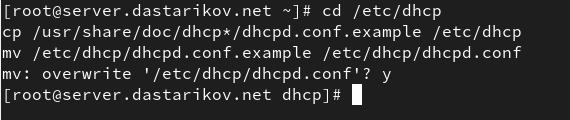
\includegraphics[width=\textwidth]{../images/image01.png}
    \captionof{figure}{Подготовка файла конфигурации.}
\end{frame}


\begin{frame}
\frametitle{Конфигурирование DHCP-сервера}
    \centering
    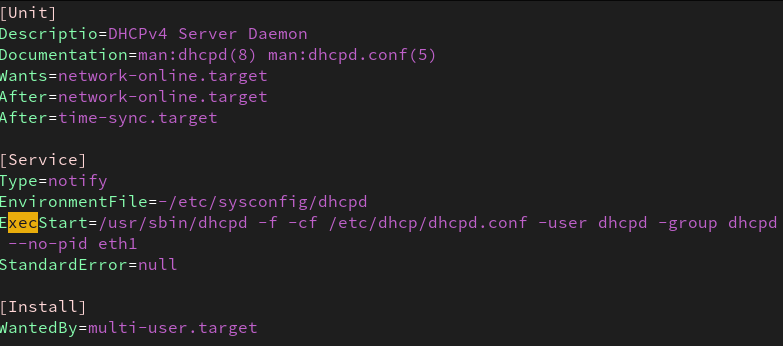
\includegraphics[width=\textwidth]{../images/image02.png}
    \captionof{figure}{Настройка dhcpd.}
\end{frame}


\begin{frame}
\frametitle{Конфигурирование DHCP-сервера}
    \centering
    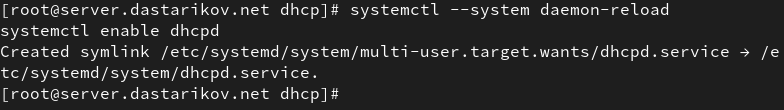
\includegraphics[width=\textwidth]{../images/image03.png}
    \captionof{figure}{Перезагрузка демона dhcpd.}
\end{frame}


\begin{frame}
\frametitle{Конфигурирование DHCP-сервера}
    \centering
    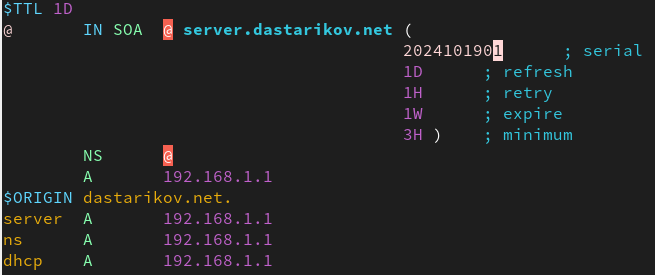
\includegraphics[width=\textwidth]{../images/image04.png}
    \captionof{figure}{Изменение файла прямой DNS-зоны.}
\end{frame}


\begin{frame}
\frametitle{Конфигурирование DHCP-сервера}
    \centering
    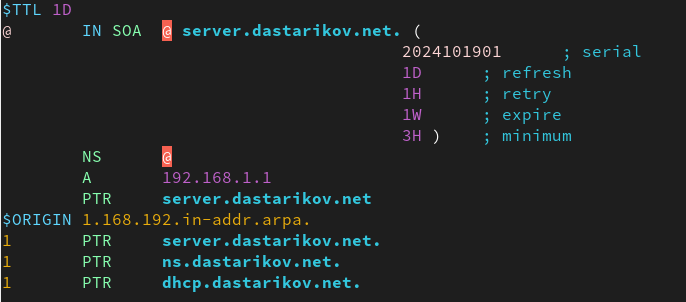
\includegraphics[width=\textwidth]{../images/image05.png}
    \captionof{figure}{Изменение файла обратной DNS-зоны.}
\end{frame}


\begin{frame}
\frametitle{Конфигурирование DHCP-сервера}
    \centering
    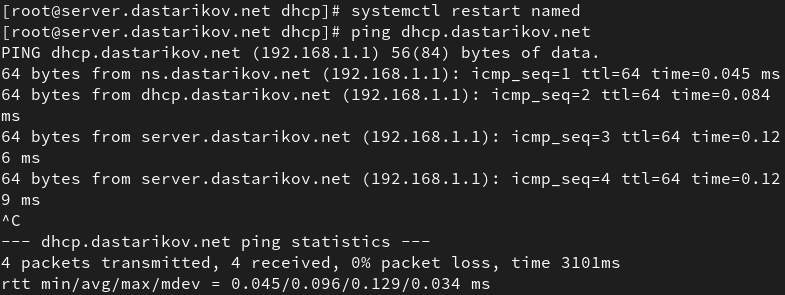
\includegraphics[width=\textwidth]{../images/image06.png}
    \captionof{figure}{Обращение к DHCP-серверу.}
\end{frame}


\begin{frame}
\frametitle{Конфигурирование DHCP-сервера}
    \centering
    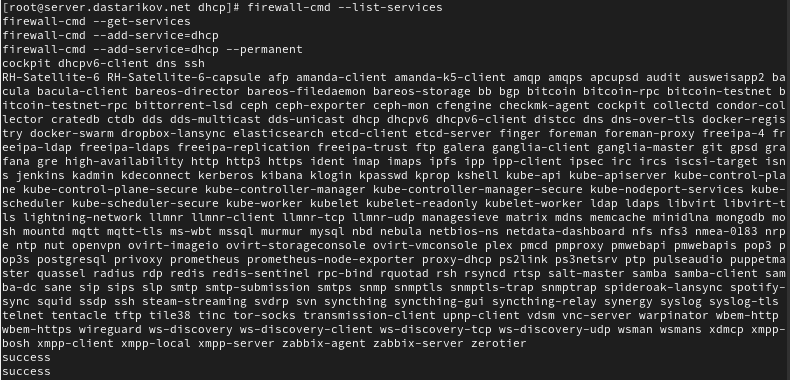
\includegraphics[width=\textwidth]{../images/image08.png}
    \captionof{figure}{Настройка межсетевого экрана для работы с DHCP.}
\end{frame}


\begin{frame}
\frametitle{Конфигурирование DHCP-сервера}
    \centering
    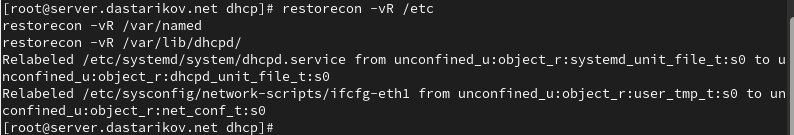
\includegraphics[width=\textwidth]{../images/image09.png}
    \captionof{figure}{Восстановление контекста безопасности SELinux.}
\end{frame}


\begin{frame}
\frametitle{Анализ работы DHCP-сервера}
    \centering
    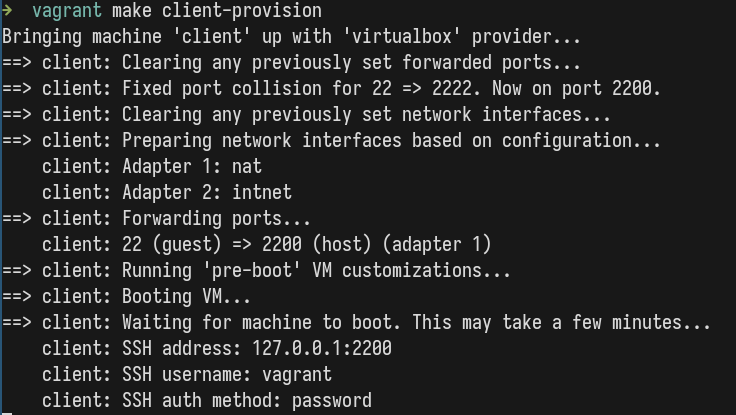
\includegraphics[width=\textwidth]{../images/image10.png}
    \captionof{figure}{Фиксирование внесенных изменений и запуск виртуальной машины client.}
\end{frame}


\begin{frame}
\frametitle{Анализ работы DHCP-сервера}
    \centering
    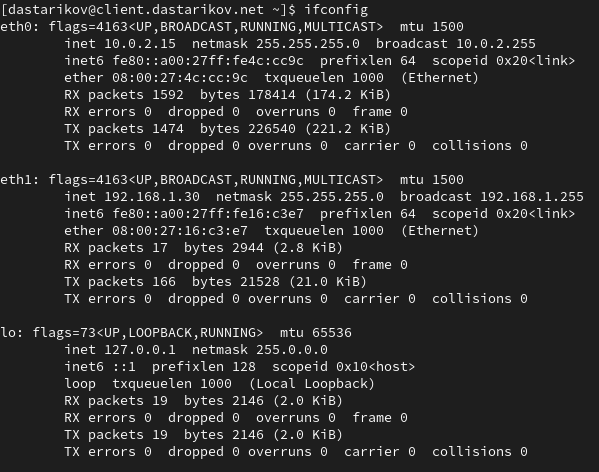
\includegraphics[width=\textwidth]{../images/image11.png}
    \captionof{figure}{Вывод информации об имеющихся интерфейсах.}
\end{frame}


\begin{frame}
\frametitle{Настройка обновления DNS-зоны}
    \centering
    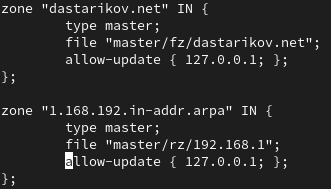
\includegraphics[width=\textwidth]{../images/image12.png}
    \captionof{figure}{Обновление файла DNS-зоны на виртуальной машине server.}
\end{frame}


\begin{frame}
\frametitle{Настройка обновления DNS-зоны}
    \centering
    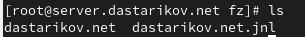
\includegraphics[width=\textwidth]{../images/image14.png}
    \captionof{figure}{Проверка создания файла.}
\end{frame}

\begin{frame}
\frametitle{Выводы}
\begin{itemize}
    \item В результате выполнения лабораторной работы приобрели практические навыки по установке и конфигурированию DHCP-сервера.
\end{itemize}
\end{frame}
\end{document}
